\section{Redes IoT e o Protocolo LoRaWAN}

As redes de Internet das Coisas (IoT) utilizam amplamente o protocolo LoRaWAN em cenários que exigem baixo consumo de energia e ampla cobertura. Embora o LoRaWAN apresente certa maturidade e conte com mecanismos de proteção continuamente aprimorados, ataques e problemas de segurança ainda afetam sua resiliência. Consequentemente, permanece necessária a evolução contínua de técnicas de prevenção e mitigação dessas ameaças \cite{hessel2023lorawan}.

%%%%%%%%%%%%%%%%%%%%%%%%%%%%%%%%%%%%%%%%%%%%%%%%%%%%

\subsection{LoRa e LoRaWAN: fundamentos e evolução do protocolo}

O LoRaWAN se destaca como uma tecnologia voltada a redes LPWAN (\textit{Low-Power Wide-Area Network}), sendo utilizado em aplicações como monitoramento remoto, agricultura inteligente e sistemas distribuídos com dispositivos embarcados. Sua proposta é permitir a comunicação entre dispositivos com baixo consumo energético, ampla cobertura e custo operacional reduzido.

É importante distinguir os termos \textit{LoRa} e \textit{LoRaWAN}, que frequentemente são tratados como sinônimos, embora representem camadas diferentes da tecnologia. O LoRa corresponde à camada física da comunicação, isto é, à técnica de modulação empregada no enlace sem fio. Já o LoRaWAN define o protocolo de comunicação acima dessa camada, estabelecendo regras para organização da rede, troca de mensagens e controle da comunicação. Em outras palavras, o LoRa fornece o meio de transmissão por rádio, enquanto o LoRaWAN define o funcionamento da rede sobre esse meio.

De forma geral, o LoRaWAN foi projetado para redes compostas por dispositivos com recursos limitados, muitas vezes alimentados por bateria e instalados em locais de difícil manutenção. Por isso, o protocolo prioriza simplicidade operacional, baixo consumo e comunicação eficiente, ainda que com taxas de transmissão menores do que tecnologias voltadas a maior vazão de dados. Essa característica o torna adequado para cenários em que pequenas quantidades de informação precisam ser transmitidas periodicamente, sem necessidade de comunicação contínua.

A evolução do LoRaWAN também é um aspecto importante. Desde sua primeira publicação, em 2015, o protocolo passou por revisões que resultaram em dois ramos principais: a família 1.0.x e a versão 1.1. As versões da família 1.0.x mantiveram interoperabilidade entre si e trouxeram principalmente correções, esclarecimentos e ajustes incrementais. Já a versão 1.1 introduziu mudanças mais relevantes, especialmente na organização de funções da rede e nos mecanismos de segurança, tornando mais clara a separação entre responsabilidades de rede e de aplicação. Neste trabalho, adota-se a família 1.0.x, uma vez que os dados utilizados na frente de aprendizado de máquina provêm de redes nas versões 1.0.3 e 1.0.4. Essa família é adotada como modelo de referência: a implementação deste trabalho utiliza a camada física LoRa em um enlace ponto a ponto, e reproduz da especificação LoRaWAN 1.0.4 \cite{lorawan104}.


\begin{figure}[htb]
  \caption{\label{lorawan_version_history}Histórico de versionamento da especificação da LoRaWAN}
  \begin{center}
      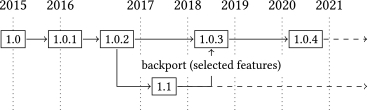
\includegraphics[scale=0.8]{barea/figuras/lorawan_version_history.png}
  \end{center}
  \legend{Fonte: \cite{hessel2023lorawan}}
\end{figure}

Mesmo com a introdução de melhorias nas versões mais recentes, a adoção de novas revisões do protocolo não ocorre de forma imediata em sistemas reais. Em aplicações IoT, sensores podem permanecer em operação por muitos anos, frequentemente sem atualização de firmware. Como consequência, versões anteriores do LoRaWAN continuam relevantes na prática, e essa coexistência entre gerações do protocolo precisa ser considerada em qualquer análise técnica ou experimental.

Assim, compreender a distinção entre LoRa e LoRaWAN, bem como a evolução do protocolo ao longo de suas versões, é essencial para analisar corretamente seu funcionamento em sistemas embarcados conectados. A partir dessa base, as próximas subseções detalham a arquitetura da rede, o processo de ativação dos dispositivos, a transferência de dados, os mecanismos de gerenciamento da comunicação e a relação dessas tecnologias com a arquitetura proposta neste trabalho.

%%%%%%%%%%%%%%%%%%%%%%%%%%%%%%%%%%%%%%%%%%%%%%%%%%%%

\subsection{A camada física LoRa}
\label{subsec:camada_fisica_lora}

O LoRa é uma técnica de modulação proprietária da Semtech, baseada em espalhamento espectral por \textit{chirp} (\textit{Chirp Spread Spectrum}, CSS). Cada símbolo é um \textit{chirp}, um sinal cuja frequência varre linearmente toda a largura de banda do canal, e a informação é codificada no instante em que essa varredura se inicia. Como a energia do símbolo é distribuída por toda a banda durante um intervalo relativamente longo, o receptor consegue correlacionar o sinal recebido com o padrão esperado mesmo quando a potência do sinal está abaixo do piso de ruído. É essa propriedade que permite sensibilidades da ordem de $-130$~dBm e enlaces de quilômetros com potências de transmissão de poucas dezenas de miliwatts \cite{semtech2015sx1276}.

Três parâmetros definem o comportamento de um enlace LoRa. O fator de espalhamento (\textit{Spreading Factor}, SF), de 7 a 12, determina quantos \textit{chirps} compõem um símbolo ($2^{\mathrm{SF}}$): cada incremento de SF dobra a duração do símbolo, aumenta a sensibilidade do receptor em cerca de 2,5~dB e reduz a taxa de dados pela metade. A largura de banda (BW), tipicamente 125, 250 ou 500~kHz, define a velocidade da varredura: bandas mais largas transmitem mais rápido e são menos sensíveis. A taxa de codificação (\textit{Coding Rate}, CR), de 4/5 a 4/8, acrescenta redundância de correção de erros ao custo de mais bits transmitidos. A Tabela~\ref{tab:parametros_lora} resume o efeito de cada parâmetro. A combinação de SF e BW define a taxa de dados (\textit{data rate}), e o LoRaWAN numera essas combinações em índices DR0 a DR6, em que DR0 corresponde à combinação mais lenta e de maior alcance.

\begin{table}[htb]
\centering
\caption{Efeito dos parâmetros da modulação LoRa}
\label{tab:parametros_lora}
\begin{tabular}{llll}
\hline
\textbf{Parâmetro} & \textbf{Ao aumentar} & \textbf{Ganha} & \textbf{Perde} \\
\hline
SF (7-12)   & 2x o tempo & sensibilidade, alcance & dados, energia/quadro \\
BW (125-500 kHz) & acelera varredura & dados & sensibilidade \\
CR (4/5-4/8) & redundância & robustez a erros & taxa útil \\
\hline
\end{tabular}
\legend{Fonte: elaborado a partir de \cite{semtech2015sx1276}.}
\end{table}

A consequência direta desses parâmetros é o tempo no ar (\textit{time on air}) de cada pacote, isto é, o intervalo durante o qual o transmissor ocupa o canal. O datasheet do transceptor \cite{semtech2015sx1276} fornece a fórmula: o tempo de símbolo é $T_s = 2^{\mathrm{SF}}/\mathrm{BW}$; o preâmbulo dura $T_{\mathrm{pre}} = (n_{\mathrm{pre}} + 4{,}25)\,T_s$, em que $n_{\mathrm{pre}}$ é o número de símbolos de preâmbulo programado; e o número de símbolos do payload é dado pela Equação~\ref{eq:npayload},

\begin{equation}
\label{eq:npayload}
n_{\mathrm{payload}} = 8 + \max\!\left( \left\lceil \frac{8\,\mathrm{PL} - 4\,\mathrm{SF} + 28 + 16\,\mathrm{CRC} - 20\,\mathrm{IH}}{4\,(\mathrm{SF} - 2\,\mathrm{DE})} \right\rceil (\mathrm{CR} + 4),\; 0 \right),
\end{equation}

\noindent em que PL é o número de bytes do payload, CRC vale 1 quando o código de verificação está habilitado, IH vale 1 quando o cabeçalho físico é omitido e DE vale 1 quando a otimização para baixas taxas (\textit{LowDataRateOptimize}) está ativa, o que o fabricante exige sempre que o tempo de símbolo ultrapassa 16~ms. O tempo no ar do pacote é $T_{\mathrm{pacote}} = T_{\mathrm{pre}} + n_{\mathrm{payload}}\,T_s$. Como $T_s$ dobra a cada incremento de SF, um mesmo pacote leva aproximadamente 25 vezes mais tempo no ar em SF12 do que em SF7. O tempo no ar determina a energia gasta por transmissão, a ocupação do canal e o tempo de exposição do quadro a interferência, e por isso é a grandeza que orienta a escolha dos parâmetros neste trabalho, apresentada no Capítulo~\ref{cap:metodo}.

O tamanho do payload é limitado em dois níveis. O campo de comprimento do pacote LoRa tem 8~bits, o que impõe o máximo físico de 255~bytes. Acima dele, os parâmetros regionais do LoRaWAN \cite{lorawan_rp002} limitam o payload de aplicação por taxa de dados, para conter o tempo no ar nas taxas mais lentas: no plano AU915, adotado no Brasil, o limite em DR0 é de 51~bytes. Um quadro que respeite esse limite pode ser transmitido em qualquer SF, inclusive nos de maior alcance.

Dois indicadores medidos pelo receptor a cada pacote descrevem a qualidade do enlace. O RSSI (\textit{Received Signal Strength Indicator}), em dBm, é a potência do sinal recebido, incluindo o ruído; valores mais próximos de zero indicam sinal mais forte. O SNR (\textit{Signal-to-Noise Ratio}), em dB, é a razão entre a potência do sinal e a do ruído; o LoRa opera com SNR negativo, até cerca de $-20$~dB em SF12, o que é justamente o que o espalhamento espectral torna possível. Em enlaces curtos e com sinal forte, o estimador de SNR do transceptor satura em torno de $+10$ a $+13$~dB e o valor deixa de variar, de modo que o SNR só se torna informativo à medida que o enlace se aproxima do seu limite de alcance. Esses dois indicadores, junto com o contador de quadros e o intervalo entre chegadas, são metadados de recepção: são produzidos pelo receptor e não dependem do conteúdo transmitido, o que os torna observáveis mesmo quando o payload é cifrado.

O LoRa opera em faixas de uso livre abaixo de 1~GHz, que variam por região. No Brasil, a ANATEL autoriza equipamentos de radiação restrita com modulação digital nas faixas de 902 a 907,5~MHz e de 915 a 928~MHz, sem necessidade de licença \cite{anatel_radiacao_restrita}. A essa segunda faixa corresponde o plano regional AU915 do LoRaWAN \cite{lorawan_rp002}, que a divide em 64 canais de \textit{uplink} de 125~kHz agrupados em oito sub-bandas, mais oito canais de 500~kHz.

Por fim, é preciso registrar o que a camada física não oferece. O LoRa define apenas a modulação e a estrutura do pacote: preâmbulo, cabeçalho físico opcional, payload e um código de verificação (CRC) de 16~bits. Não há endereçamento, controle de acesso ao meio nem qualquer mecanismo de segurança. O CRC detecta erros de transmissão, mas pode ser recalculado por qualquer parte, e portanto não protege contra modificação, forja ou repetição de quadros. No LoRaWAN, essas funções são acrescentadas pela camada MAC, que define endereços, contadores e a proteção criptográfica do quadro com AES-128 no modo CTR para confidencialidade e AES-CMAC para o código de integridade \cite{lorawan104}. Em um enlace que utilize apenas a camada física LoRa, tudo o que está acima dela precisa ser fornecido pela aplicação. Essa constatação fundamenta a arquitetura adotada neste trabalho, discutida na Subseção~\ref{subsec:implicacoes_arquitetura}.


%%%%%%%%%%%%%%%%%%%%%%%%%%%%%%%%%%%%%%%%%%%%%%%%%%%%

\subsection{Arquitetura da Rede}

A arquitetura do LoRaWAN é composta por diferentes entidades, cada uma com uma função específica no funcionamento da rede. De forma geral, os dispositivos finais, chamados de \textit{End Devices}, são responsáveis por coletar e transmitir dados. Esses dispositivos se comunicam por rádio com um ou mais \textit{Gateways}, que atuam como pontes entre a rede LoRa e a infraestrutura conectada por IP. Os gateways, por sua vez, apenas recebem os quadros transmitidos pelos dispositivos e os encaminham para os servidores da rede, sem realizar processamento completo do protocolo. \cite{hessel2023lorawan}

Essa organização forma uma topologia conhecida como \textit{star-of-stars}. Nela, os dispositivos finais não se comunicam diretamente entre si, e também não estabelecem vínculo fixo com um único gateway. Em vez disso, uma mesma transmissão pode ser recebida por vários gateways que estejam dentro de alcance. Essa característica aumenta a cobertura da rede e oferece maior robustez na recepção das mensagens, especialmente em cenários distribuídos e com mobilidade.

\begin{figure}[htb]
  \caption{\label{lorawan_architeture}Arquitetura de rede LoRaWAN}
  \begin{center}
      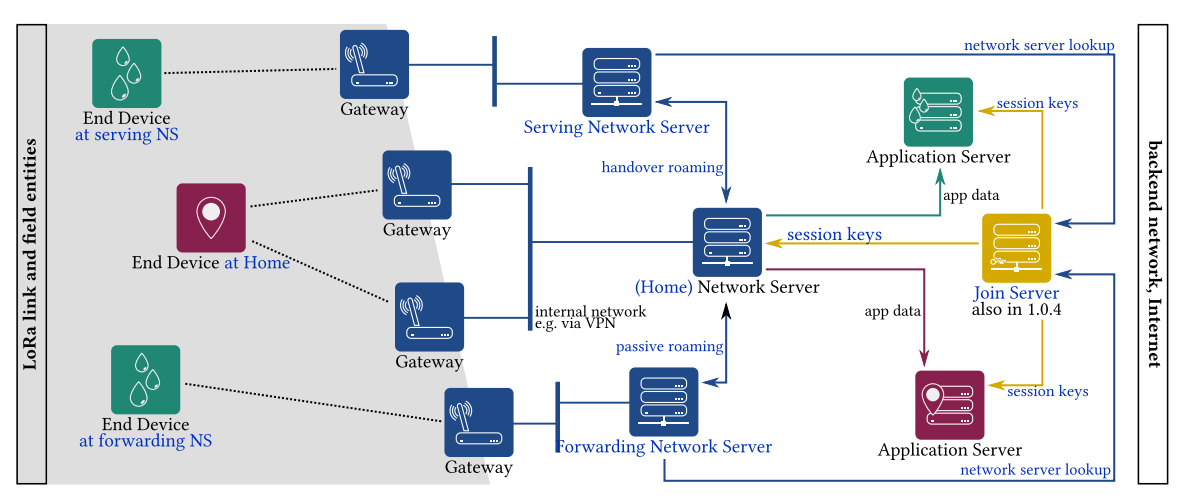
\includegraphics[scale=0.4]{barea/figuras/architeture_LoRaWan.png}
  \end{center}
  \legend{Fonte: \cite{hessel2023lorawan}}
\end{figure}

Após o encaminhamento feito pelos gateways, as mensagens chegam ao \textit{Network Server}. Esse servidor exerce papel central na rede, pois é responsável por processar as mensagens recebidas, eliminar duplicidades causadas pela recepção do mesmo quadro por múltiplos gateways, validar a integridade das mensagens e executar as funções de gerenciamento da camada MAC. Em outras palavras, é o \textit{Network Server} que coordena o funcionamento lógico da rede LoRaWAN.

Os dados de aplicação seguem então para o \textit{Application Server}, que é o componente responsável por tratar a informação útil transportada pelo dispositivo final. É nesse servidor que os dados recebidos podem ser decifrados, interpretados e encaminhados para a aplicação de interesse, como um sistema de monitoramento, um banco de dados ou uma plataforma de análise. Essa separação entre funções de rede e funções de aplicação é importante porque organiza melhor as responsabilidades do sistema e reduz o acoplamento entre comunicação e processamento da informação.

Na evolução do protocolo, especialmente a partir do LoRaWAN 1.1, o \textit{Join Server} passa a ter um papel mais explícito na arquitetura. Esse componente participa do processo de ativação dos dispositivos e da derivação de chaves de sessão, contribuindo para uma separação mais clara entre gerenciamento de rede e segurança da aplicação. Com isso, a arquitetura do LoRaWAN se torna mais organizada do ponto de vista funcional e mais adequada a cenários em que diferentes operadores ou domínios de serviço precisam cooperar.

Assim, a arquitetura do LoRaWAN pode ser entendida como uma organização em camadas funcionais: o dispositivo final coleta e transmite os dados, o gateway encaminha os quadros recebidos, o \textit{Network Server} gerencia a comunicação da rede, e o \textit{Application Server} entrega os dados à aplicação. Nas versões mais recentes, o \textit{Join Server} complementa essa estrutura ao apoiar o processo de ativação e gerenciamento de chaves. Essa divisão de papéis é fundamental para compreender como o protocolo opera e como seus componentes podem ser relacionados à arquitetura proposta neste trabalho.

%%%%%%%%%%%%%%%%%%%%%%%%%%%%%%%%%%%%%%%%%%%%%%%%%%%%

\subsection{Ativação do Dispositivo}

Antes de transmitir dados de aplicação, um dispositivo LoRaWAN precisa ser ativado na rede. Esse processo define como o dispositivo passa a ser reconhecido pelo sistema e como obtém o contexto necessário para a comunicação, incluindo identificadores, parâmetros de sessão e chaves utilizadas ao longo da operação. De forma geral, o LoRaWAN admite dois modos principais de ativação: \textit{Activation By Personalization} (ABP) e \textit{Over-The-Air Activation} (OTAA). \cite{hessel2023lorawan}

No modo ABP, o dispositivo já é configurado previamente com os parâmetros de sessão necessários para operar. Assim, ele pode iniciar a transmissão diretamente, sem realizar um procedimento de ingresso na rede a cada inicialização. Essa abordagem é mais simples do ponto de vista de implementação, mas oferece menor flexibilidade operacional, já que os parâmetros de comunicação ficam previamente fixados no dispositivo.

No modo OTAA, por outro lado, o dispositivo realiza um procedimento de ingresso na rede antes de iniciar sua operação normal. Nesse processo, o nó envia uma solicitação de ativação e, a partir da resposta da infraestrutura da rede, passa a operar com parâmetros e chaves de sessão derivados especificamente para aquela conexão. Em comparação com o ABP, essa abordagem é mais flexível e mais adequada a cenários reais, pois facilita renovação de chaves, adaptação do contexto de comunicação e suporte a funcionalidades mais avançadas do protocolo.

De forma simplificada, a ativação por OTAA envolve a troca de mensagens de ingresso e a geração de chaves de sessão a partir de credenciais previamente associadas ao dispositivo. Esse mecanismo permite que a rede estabeleça uma nova sessão de comunicação de forma controlada, em vez de depender sempre de parâmetros estáticos. Por esse motivo, o OTAA tende a ser considerado a alternativa mais robusta para implantações práticas, especialmente quando se deseja maior controle do ciclo de vida dos dispositivos e melhor suporte a segurança.

\begin{figure}[htb]
  \caption{\label{lorawan_join_process} (a) OTAA processo de entrada LoRaWAN 1.0.x. (b) OTAA processo de entrada LoRaWAN 1.1}
  \begin{center}
      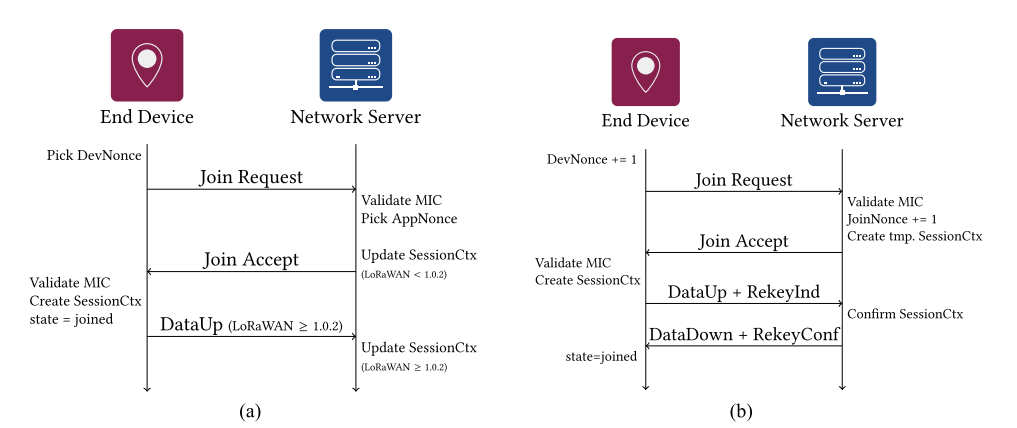
\includegraphics[scale=0.4]{barea/figuras/otaa_join_process.png}
  \end{center}
  \legend{Fonte: \cite{hessel2023lorawan}}
\end{figure}

A evolução do protocolo também impacta esse processo. Nas versões da família 1.0.x, a ativação já podia ocorrer por ABP ou OTAA, mas a versão 1.1 introduziu uma separação mais clara entre funções de rede e aplicação, além de mudanças no tratamento das chaves e no papel do \textit{Join Server}. Com isso, o processo de ativação passou a ser mais estruturado e alinhado com uma arquitetura de segurança mais organizada.

Assim, a ativação do dispositivo representa uma etapa fundamental no funcionamento do LoRaWAN, pois estabelece as condições iniciais para que a comunicação ocorra de forma válida dentro da rede. Enquanto o ABP oferece uma alternativa mais simples, o OTAA apresenta maior flexibilidade e melhor aderência a cenários práticos e escaláveis. A partir dessa etapa, o dispositivo pode iniciar a troca de dados com a infraestrutura da rede, conforme discutido na próxima subseção.

%%%%%%%%%%%%%%%%%%%%%%%%%%%%%%%%%%%%%%%%%%%%%%%%%%%%

\subsection{Transferência de Dados}

Após a ativação do dispositivo, a comunicação de dados pode ocorrer entre o dispositivo final e a infraestrutura da rede. No LoRaWAN, as mensagens enviadas pelo dispositivo em direção à rede são chamadas de \textit{DataUp}, enquanto as mensagens enviadas pela rede ao dispositivo são chamadas de \textit{Datadown}. Essa troca de dados pode ocorrer de forma simples, apenas com envio da informação, ou com solicitação de confirmação de recebimento, dependendo da necessidade da aplicação. \cite{hessel2023lorawan}

Quando não há necessidade de confirmação, utilizam-se mensagens não confirmadas, que reduzem o overhead da comunicação e tendem a ser mais adequadas a aplicações periódicas de monitoramento. Já nas mensagens confirmadas, a camada MAC pode exigir uma resposta da rede, permitindo ao dispositivo verificar se a transmissão foi reconhecida. Essa distinção é importante porque envolve um compromisso entre confiabilidade e consumo de recursos, já que confirmações adicionais aumentam o uso do canal e o gasto energético.

\begin{figure}[htb]
  \caption{\label{lorawan_message_ed}Classe para comunicacoes ED}
  \begin{center}
      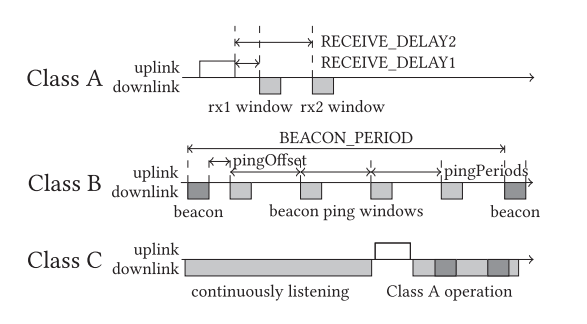
\includegraphics[scale=0.6]{barea/figuras/ed_operations_class.png}
  \end{center}
  \legend{Fonte: \cite{hessel2023lorawan}}
\end{figure}

O LoRaWAN define três modos principais de operação para os dispositivos finais, chamados de classes A, B e C. A Classe A é a padrão e está presente em todos os dispositivos LoRaWAN. Nela, o dispositivo inicia a comunicação por meio de um \textit{uplink} e, após essa transmissão, abre duas pequenas janelas de recepção para possíveis mensagens de \textit{downlink}. Essas janelas são conhecidas como RX1 e RX2. Esse modelo é o mais eficiente em termos energéticos, pois o dispositivo permanece a maior parte do tempo fora de escuta. 

Na Classe B, além do comportamento básico da Classe A, o dispositivo sincroniza sua operação com sinais periódicos da rede e passa a abrir janelas adicionais de recepção em instantes programados. Isso permite maior previsibilidade para o envio de mensagens em \textit{downlink}, embora aumente a complexidade da operação. Já na Classe C, o dispositivo permanece praticamente em escuta contínua, fechando a recepção apenas quando transmite. Essa abordagem reduz a latência de \textit{downlink}, mas aumenta significativamente o consumo de energia, sendo mais adequada a dispositivos com menor restrição energética.

\begin{figure}[htb]
  \caption{\label{messages_abc} Estrutura e Criptografia das mensagems LoRaWan}
    \begin{center}
      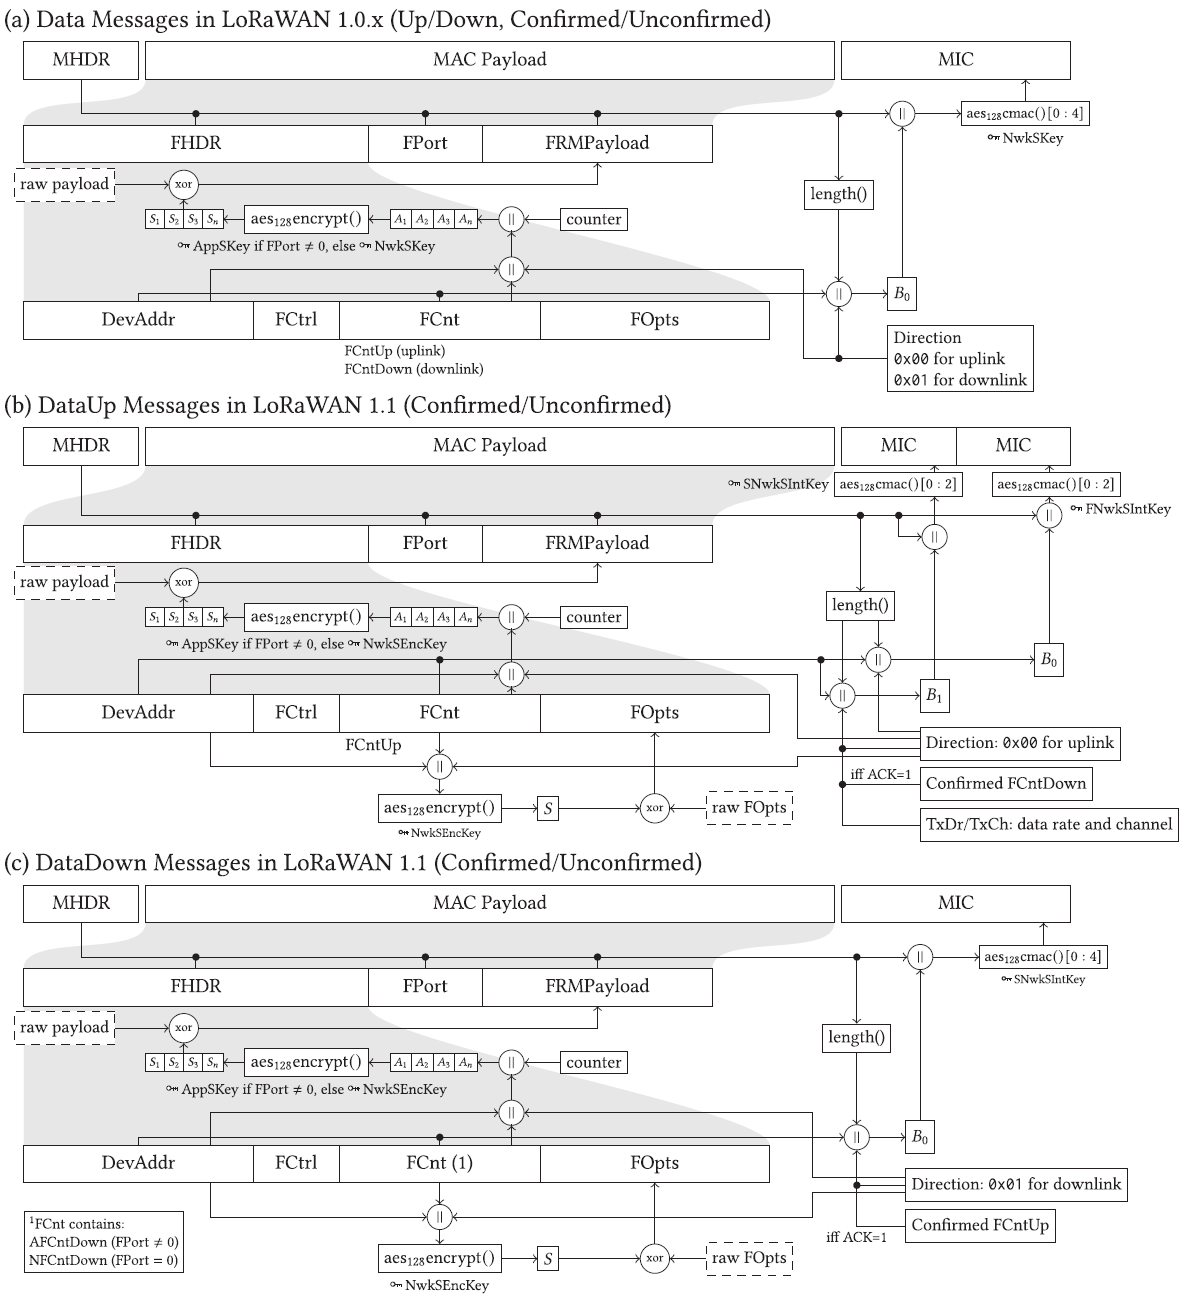
\includegraphics[scale=0.3]{barea/figuras/structure_messages_abc.png}
  \end{center}
  \legend{Fonte: \cite{hessel2023lorawan}}
\end{figure}

As mensagens de dados do LoRaWAN possuem uma estrutura padronizada. De forma geral, elas incluem um cabeçalho com a identificação do tipo de mensagem, um cabeçalho de quadro com informações de controle e endereçamento, um contador de quadros e o campo destinado à carga útil da aplicação. Entre esses elementos, o contador de quadros, representado por \textit{FCnt}, é especialmente importante para o acompanhamento da sequência das mensagens. Outros campos, como \textit{FPort} e \textit{FOpts}, ajudam a distinguir dados de aplicação e informações de controle da rede. Além disso, as mensagens incluem um código de integridade, chamado \textit{MIC}, utilizado para verificação da validade da comunicação.

De modo geral, a transferência de dados no LoRaWAN foi projetada para equilibrar simplicidade, baixo consumo e capacidade de operação em redes distribuídas de longo alcance. A existência de diferentes classes de operação e de mecanismos para mensagens confirmadas ou não confirmadas permite adaptar o comportamento da comunicação às necessidades da aplicação. A partir dessa base, torna-se possível compreender melhor como a rede ajusta e gerencia sua operação, tema discutido na próxima subseção.

%%%%%%%%%%%%%%%%%%%%%%%%%%%%%%%%%%%%%%%%%%%%%%%%%%%%

\subsection{Gerenciamento da Rede}

Como o LoRaWAN é um protocolo de camada MAC voltado a redes LPWAN, ele precisa de mecanismos para configurar dispositivos, ajustar parâmetros de comunicação e acompanhar o estado da rede. Parte dessas funções já aparece diretamente nos próprios campos das mensagens, como endereços, contadores de quadros e confirmações. No entanto, o protocolo também define comandos específicos para gerenciamento, conhecidos como \textit{MAC commands}, que permitem trocar informações de controle entre o dispositivo final e a infraestrutura da rede. \cite{hessel2023lorawan}

Esses comandos são usados para diferentes finalidades de operação. Entre elas, estão a obtenção de informações sobre a qualidade da conexão, o ajuste de parâmetros de transmissão e a sincronização de tempo. Assim, o gerenciamento da rede não ocorre como uma função separada do restante do protocolo, mas sim como parte do próprio fluxo de comunicação entre os dispositivos e os servidores da rede. 

Entre os mecanismos de gerenciamento, um dos mais importantes é o \textit{Adaptive Data Rate} (ADR). O ADR tem como objetivo ajustar a taxa de transmissão de dados e outros parâmetros de rádio de acordo com as condições de comunicação observadas na rede. Na prática, isso permite definir combinações mais adequadas de \textit{Spreading Factor}, largura de banda e potência de transmissão, buscando equilibrar confiabilidade, consumo de energia e uso eficiente do meio de comunicação.

De forma geral, o gerenciamento da rede no LoRaWAN existe para manter a comunicação funcional e eficiente ao longo do tempo. Por meio de comandos de controle e mecanismos como o ADR, o protocolo consegue ajustar seu comportamento às condições reais de operação, o que é especialmente importante em ambientes distribuídos, sujeitos a variações de alcance, interferência e disponibilidade energética. Com essa base conceitual, torna-se possível avançar para uma análise mais voltada à forma como essas tecnologias serão utilizadas na arquitetura proposta neste trabalho.

%%%%%%%%%%%%%%%%%%%%%%%%%%%%%%%%%%%%%%%%%%%%%%%%%%%%

\subsection{LoRa versus Wi-Fi no contexto do projeto}

Embora LoRa e Wi-Fi sejam tecnologias de comunicação sem fio, elas atendem a necessidades diferentes e, neste trabalho, não são tratadas como soluções concorrentes. Cada uma delas ocupa um papel específico na arquitetura proposta, de acordo com suas características de alcance, consumo energético, taxa de transmissão e facilidade de integração com os demais componentes do sistema.

O LoRa foi projetado para aplicações de longo alcance e baixo consumo, sendo adequado a dispositivos embarcados que operam com recursos limitados e transmitem pequenas quantidades de dados de forma periódica ou eventual. Essas características o tornam compatível com o cenário deste projeto, no qual o nó sensor precisa operar de forma eficiente, com comunicação sem fio e possibilidade de instalação afastada do ponto central da rede.

O Wi-Fi, por outro lado, oferece maior taxa de transmissão e integração mais direta com redes IP e serviços de aplicação, como APIs e servidores de armazenamento. Em contrapartida, apresenta maior consumo energético e menor adequação a nós distribuídos que precisem operar por longos períodos com restrição de energia. Por esse motivo, o Wi-Fi não foi adotado como tecnologia principal de comunicação entre os nós embarcados e a infraestrutura de campo.

No contexto deste trabalho, a solução adotada combina as duas tecnologias de forma complementar. O trecho entre o nó sensor e o \textit{gateway} utiliza LoRa em enlace ponto a ponto, preservando as vantagens de alcance e baixo consumo no nível embarcado. Já o trecho entre o \textit{gateway} e o servidor utiliza Wi-Fi, aproveitando sua integração mais simples com a infraestrutura de rede e com os serviços responsáveis por receber, armazenar e processar os dados coletados.

Essa divisão permite separar dois problemas distintos dentro da arquitetura. O primeiro é a comunicação entre dispositivos embarcados em campo, em que baixo consumo e cobertura são requisitos centrais. O segundo é a entrega dos dados para uma camada de processamento e persistência, em que a prioridade passa a ser conectividade com a rede local ou com a Internet, além da facilidade de integração com a aplicação. Assim, a escolha conjunta de LoRa e Wi-Fi não representa uma sobreposição de tecnologias, mas sim uma composição coerente entre camadas com funções diferentes.

Dessa forma, o uso de LoRa no trecho embarcado e de Wi-Fi no trecho de retaguarda estabelece uma arquitetura compatível com os objetivos do projeto. Ao mesmo tempo em que preserva as vantagens de uma rede LPWAN na comunicação entre os dispositivos de campo, essa abordagem também facilita a construção da interface com o servidor, a persistência dos dados e a futura integração com mecanismos de análise e segurança.

%%%%%%%%%%%%%%%%%%%%%%%%%%%%%%%%%%%%%%%%%%%%%%%%%%%%

\subsection{Implicações para a arquitetura proposta}
\label{subsec:implicacoes_arquitetura}

Os conceitos apresentados nas subseções anteriores permitem situar a arquitetura adotada neste trabalho. No projeto proposto, o nó sensor opera como dispositivo final, responsável pela coleta de dados do ambiente e pela transmissão dessas informações pela rede sem fio. Essa comunicação ocorre por um enlace LoRa ponto a ponto entre o nó e o \textit{gateway}, explorando as características de longo alcance e baixo consumo da camada física.

O gateway exerce o papel de ponto de transição entre a rede de campo e a infraestrutura de retaguarda. Sua função principal é receber os quadros enviados pelos dispositivos finais e encaminhá-los para a camada de processamento do sistema. A partir desse ponto, os dados podem ser entregues a um servidor ou API responsável por armazenamento, organização e disponibilização das informações para etapas posteriores de análise.

Essa divisão é importante porque separa o problema da comunicação embarcada do problema de processamento dos dados. No nível dos nós em campo, o foco está em transmitir com eficiência, respeitando restrições de energia, alcance e capacidade computacional. Já no nível do gateway e do servidor, torna-se possível concentrar funções de persistência, observabilidade e integração com serviços de aplicação, sem impor esse custo diretamente aos dispositivos finais.

A opção pelo enlace ponto a ponto, em lugar de uma rede LoRaWAN completa, é uma decisão de projeto, e não apenas uma consequência do hardware disponível. Uma rede LoRaWAN exige \textit{gateway} multicanal e \textit{network server}, e sua camada MAC determina o uso de AES-128 para proteger todo quadro. Nesse contexto, a inserção de outra primitiva criptográfica seria redundante, e a comparação entre algoritmos perderia sentido. O enlace ponto a ponto, ao contrário, deixa a camada acima da física inteiramente sob controle da aplicação, o que abre o espaço de projeto no qual a escolha do algoritmo de criptografia autenticada pode ser feita e avaliada. Além disso, controlar as duas pontas do enlace permite conhecer o instante e o conteúdo de cada transmissão, condição necessária para rotular o que é operação normal e o que é anomalia.

O LoRaWAN permanece como modelo de referência. Os papéis de \textit{gateway}, \textit{network server} e \textit{application server}, separados na arquitetura da Figura~\ref{lorawan_architeture}, são aqui concentrados em um único dispositivo, o \textit{gateway}, que recebe, valida e encaminha os quadros. A estrutura do quadro transmitido segue a do PHYPayload da especificação 1.0.4: o identificador do dispositivo e o contador de quadros vão em claro, e a alteração de qualquer um dos dois invalida o código de autenticação que encerra o quadro, depois do \textit{payload} cifrado. O esquema de provisionamento equivale à ativação por personalização (ABP), com chave e identificador gravados no dispositivo e sem procedimento de ingresso. O formato do quadro e a ordem de validação implementados são descritos na Subseção~\ref{subsec:implementacao_infra}.

Como discutido na Subseção~\ref{subsec:camada_fisica_lora}, a camada física LoRa não oferece nenhum mecanismo de segurança, e em um enlace ponto a ponto não existe a camada MAC do LoRaWAN que os forneceria. A proteção do quadro contra leitura, modificação, forja e repetição precisa, portanto, ser fornecida pela própria aplicação. Ao mesmo tempo, a presença de dados trafegando entre o dispositivo embarcado, o \textit{gateway} e a infraestrutura de \textit{backend} exige que a proteção seja pensada para cada trecho, e não apenas para o enlace de rádio.

Além disso, a própria dinâmica operacional da rede produz informações que podem ser úteis para análise de comportamento, identificação de falhas e detecção de atividades anômalas. Parâmetros de transmissão, padrões temporais de envio e eventos observados na comunicação podem servir como base para uma camada adicional de monitoramento do sistema, complementando a proteção oferecida pelos mecanismos tradicionais do protocolo.

Dessa forma, a arquitetura proposta neste trabalho não se limita ao transporte de dados entre dispositivos e servidor. Ela também cria as condições para incorporar camadas complementares de segurança e análise. Nesse contexto, a próxima seção discute o uso de criptografia leve como mecanismo adequado à proteção de dados em dispositivos com recursos restritos, enquanto a seção seguinte apresenta o papel do \textit{Machine Learning} como apoio à análise do comportamento da rede e à detecção de anomalias.


%%%%%%%%%%%%%%%%%%%%%%%%%%%%%%%%%%%%%%%%%%%%%%%%%%%%
%%%%%%%%%%%%%%%%%%%%%%%%%%%%%%%%%%%%%%%%%%%%%%%%%%%%
